\documentclass{article}\usepackage[]{graphicx}\usepackage[]{color}
%% maxwidth is the original width if it is less than linewidth
%% otherwise use linewidth (to make sure the graphics do not exceed the margin)
\makeatletter
\def\maxwidth{ %
  \ifdim\Gin@nat@width>\linewidth
    \linewidth
  \else
    \Gin@nat@width
  \fi
}
\makeatother

\definecolor{fgcolor}{rgb}{0.345, 0.345, 0.345}
\newcommand{\hlnum}[1]{\textcolor[rgb]{0.686,0.059,0.569}{#1}}%
\newcommand{\hlstr}[1]{\textcolor[rgb]{0.192,0.494,0.8}{#1}}%
\newcommand{\hlcom}[1]{\textcolor[rgb]{0.678,0.584,0.686}{\textit{#1}}}%
\newcommand{\hlopt}[1]{\textcolor[rgb]{0,0,0}{#1}}%
\newcommand{\hlstd}[1]{\textcolor[rgb]{0.345,0.345,0.345}{#1}}%
\newcommand{\hlkwa}[1]{\textcolor[rgb]{0.161,0.373,0.58}{\textbf{#1}}}%
\newcommand{\hlkwb}[1]{\textcolor[rgb]{0.69,0.353,0.396}{#1}}%
\newcommand{\hlkwc}[1]{\textcolor[rgb]{0.333,0.667,0.333}{#1}}%
\newcommand{\hlkwd}[1]{\textcolor[rgb]{0.737,0.353,0.396}{\textbf{#1}}}%
\let\hlipl\hlkwb

\usepackage{framed}
\makeatletter
\newenvironment{kframe}{%
 \def\at@end@of@kframe{}%
 \ifinner\ifhmode%
  \def\at@end@of@kframe{\end{minipage}}%
  \begin{minipage}{\columnwidth}%
 \fi\fi%
 \def\FrameCommand##1{\hskip\@totalleftmargin \hskip-\fboxsep
 \colorbox{shadecolor}{##1}\hskip-\fboxsep
     % There is no \\@totalrightmargin, so:
     \hskip-\linewidth \hskip-\@totalleftmargin \hskip\columnwidth}%
 \MakeFramed {\advance\hsize-\width
   \@totalleftmargin\z@ \linewidth\hsize
   \@setminipage}}%
 {\par\unskip\endMakeFramed%
 \at@end@of@kframe}
\makeatother

\definecolor{shadecolor}{rgb}{.97, .97, .97}
\definecolor{messagecolor}{rgb}{0, 0, 0}
\definecolor{warningcolor}{rgb}{1, 0, 1}
\definecolor{errorcolor}{rgb}{1, 0, 0}
\newenvironment{knitrout}{}{} % an empty environment to be redefined in TeX

\usepackage{alltt}
\IfFileExists{upquote.sty}{\usepackage{upquote}}{}
\begin{document}



\begin{knitrout}
\definecolor{shadecolor}{rgb}{0.969, 0.969, 0.969}\color{fgcolor}\begin{kframe}
\begin{alltt}
\hlcom{## Load libraries}
\hlkwd{library}\hlstd{(splines)}
\hlkwd{library}\hlstd{(MASS)}

\hlkwd{library}\hlstd{(doParallel)} \hlcom{##to make cluster (on Windows)}
\end{alltt}


{\ttfamily\noindent\itshape\color{messagecolor}{\#\# Loading required package: foreach}}

{\ttfamily\noindent\itshape\color{messagecolor}{\#\# Loading required package: iterators}}

{\ttfamily\noindent\itshape\color{messagecolor}{\#\# Loading required package: parallel}}\begin{alltt}
\hlkwd{library}\hlstd{(foreach)} \hlcom{##to use foreach function that does the parallel processing}
\hlkwd{library}\hlstd{(doRNG)} \hlcom{##for reproducible seeds when doing parallel processing}
\end{alltt}


{\ttfamily\noindent\itshape\color{messagecolor}{\#\# Loading required package: rngtools}}

{\ttfamily\noindent\itshape\color{messagecolor}{\#\# Loading required package: pkgmaker}}

{\ttfamily\noindent\itshape\color{messagecolor}{\#\# Loading required package: registry}}

{\ttfamily\noindent\itshape\color{messagecolor}{\#\# \\\#\# Attaching package: 'pkgmaker'}}

{\ttfamily\noindent\itshape\color{messagecolor}{\#\# The following object is masked from 'package:base':\\\#\# \\\#\#\ \ \ \  isNamespaceLoaded}}\begin{alltt}
\hlcom{##Source functions}
\hlkwd{source}\hlstd{(}\hlstr{"../functions.R"}\hlstd{)}

\hlcom{## Define the number of tests}
\hlstd{ntest} \hlkwb{<-} \hlnum{10000}

\hlcom{## Set number of simulations}
\hlstd{nSims} \hlkwb{<-} \hlnum{200}
\end{alltt}
\end{kframe}
\end{knitrout}

Do the simulations for a variety of alternative distributions:
\begin{knitrout}
\definecolor{shadecolor}{rgb}{0.969, 0.969, 0.969}\color{fgcolor}\begin{kframe}
\begin{alltt}
\hlstd{alts} \hlkwb{<-} \hlkwd{c}\hlstd{(}\hlstr{"alt_beta"}\hlstd{,}\hlstr{"alt_chisq_large_3_3"}\hlstd{,}\hlstr{"alt_chisq_large"}\hlstd{,}
          \hlstr{"alt_chisq_small_3_3"}\hlstd{,}\hlstr{"alt_chisq_small"}\hlstd{,}
          \hlstr{"alt_t_large"}\hlstd{,}\hlstr{"alt_t_small"}\hlstd{,}
          \hlstr{"alt_z_large"}\hlstd{,}
          \hlstr{"alt_z_small"}\hlstd{)}
\end{alltt}
\end{kframe}
\end{knitrout}

\section{Probability of being a false positive is flat}

\begin{knitrout}
\definecolor{shadecolor}{rgb}{0.969, 0.969, 0.969}\color{fgcolor}\begin{kframe}
\begin{alltt}
\hlcom{## Set up the time vector and the probability of being null}
\hlstd{tme} \hlkwb{<-} \hlkwd{seq}\hlstd{(}\hlnum{0}\hlstd{,}\hlnum{1}\hlstd{,} \hlkwc{length}\hlstd{=ntest)}
\hlstd{pi0} \hlkwb{<-} \hlkwd{rep}\hlstd{(}\hlnum{0.9}\hlstd{,} \hlkwc{length}\hlstd{=ntest)}

\hlkwd{plot}\hlstd{(pi0} \hlopt{~} \hlstd{tme)}

\hlkwa{for}\hlstd{(alt} \hlkwa{in} \hlstd{alts)}
\hlstd{\{}
  \hlstd{pValuesSims} \hlkwb{<-} \hlkwd{run_sims_alt}\hlstd{(alt, nSims, pi0)}

  \hlstd{zValuesSims} \hlkwb{<-} \hlstd{pValuesSims[,(}\hlnum{2}\hlopt{*}\hlstd{ntest}\hlopt{+}\hlnum{1}\hlstd{)}\hlopt{:}\hlstd{(}\hlnum{3}\hlopt{*}\hlstd{ntest)]}
  \hlstd{nullHypSims} \hlkwb{<-} \hlstd{pValuesSims[,(ntest}\hlopt{+}\hlnum{1}\hlstd{)}\hlopt{:}\hlstd{(}\hlnum{2}\hlopt{*}\hlstd{ntest)]}
  \hlstd{pValuesSims} \hlkwb{<-} \hlstd{pValuesSims[,}\hlnum{1}\hlopt{:}\hlstd{ntest]}

  \hlcom{##save results}
  \hlkwd{save}\hlstd{(}\hlkwc{file}\hlstd{=}\hlkwd{paste}\hlstd{(alt,} \hlstr{"simResults_1.RData"}\hlstd{,}\hlkwc{sep}\hlstd{=}\hlstr{"/"}\hlstd{),}
       \hlkwc{list}\hlstd{=}\hlkwd{c}\hlstd{(}\hlstr{"pi0"}\hlstd{,} \hlstr{"tme"}\hlstd{,} \hlstr{"nullHypSims"}\hlstd{,}\hlstr{"pValuesSims"}\hlstd{,}\hlstr{"zValuesSims"}\hlstd{))}
\hlstd{\}}
\end{alltt}
\end{kframe}

{\centering 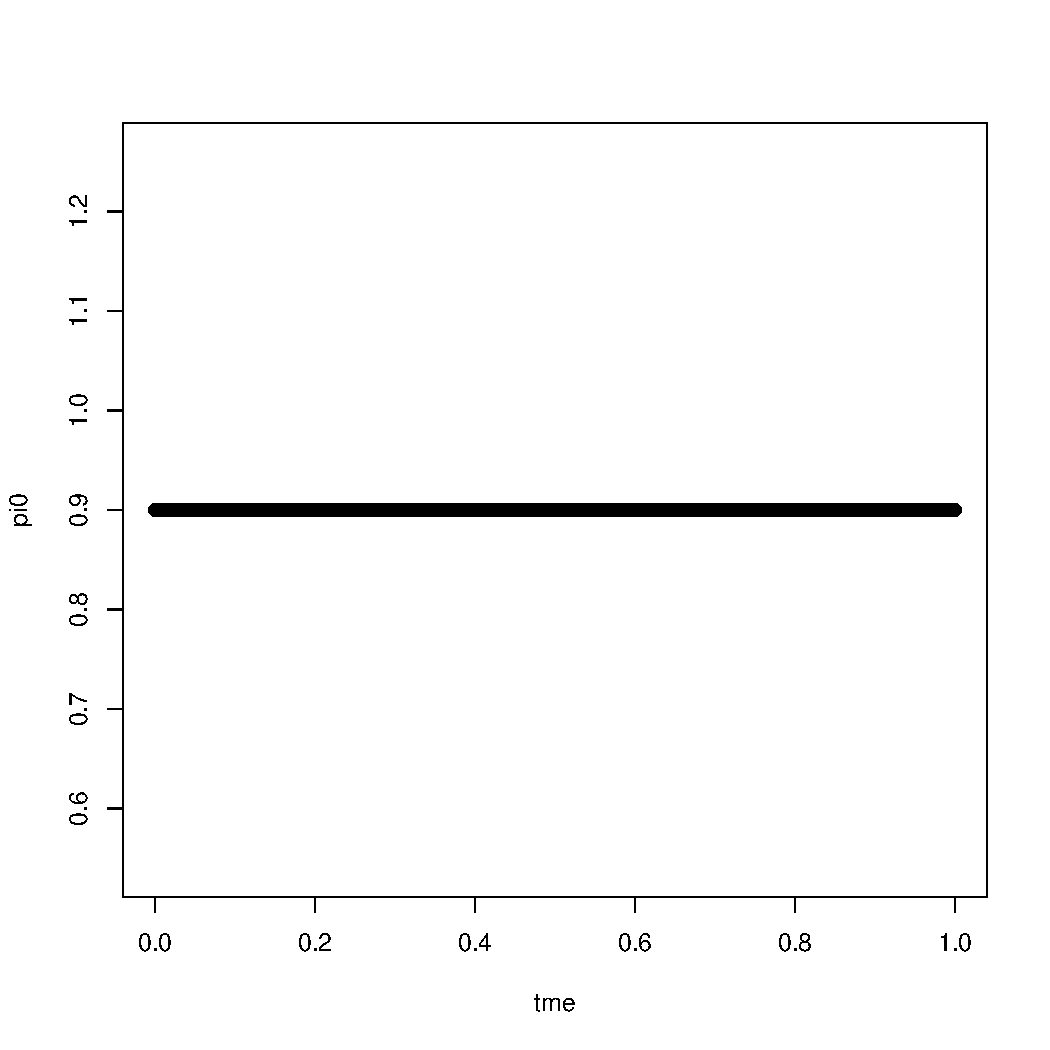
\includegraphics[width=\maxwidth]{Figures/I-1} 

}



\end{knitrout}

\section{Probability of being a false positive is smooth in one variable}

\begin{knitrout}
\definecolor{shadecolor}{rgb}{0.969, 0.969, 0.969}\color{fgcolor}\begin{kframe}
\begin{alltt}
\hlcom{## Set up the time vector and the probability of being null}
\hlstd{tme} \hlkwb{<-} \hlkwd{seq}\hlstd{(}\hlnum{0}\hlstd{,}\hlnum{1}\hlstd{,} \hlkwc{length}\hlstd{=ntest)}
\hlstd{pi0} \hlkwb{<-} \hlkwd{fSingle}\hlstd{(tme)}

\hlkwd{plot}\hlstd{(pi0} \hlopt{~} \hlstd{tme)}

\hlkwa{for}\hlstd{(alt} \hlkwa{in} \hlstd{alts)}
\hlstd{\{}
  \hlstd{pValuesSims} \hlkwb{<-} \hlkwd{run_sims_alt}\hlstd{(alt, nSims, pi0)}

  \hlkwd{dim}\hlstd{(pValuesSims)}

  \hlstd{zValuesSims} \hlkwb{<-} \hlstd{pValuesSims[,(}\hlnum{2}\hlopt{*}\hlstd{ntest}\hlopt{+}\hlnum{1}\hlstd{)}\hlopt{:}\hlstd{(}\hlnum{3}\hlopt{*}\hlstd{ntest)]}
  \hlstd{nullHypSims} \hlkwb{<-} \hlstd{pValuesSims[,(ntest}\hlopt{+}\hlnum{1}\hlstd{)}\hlopt{:}\hlstd{(}\hlnum{2}\hlopt{*}\hlstd{ntest)]}
  \hlstd{pValuesSims} \hlkwb{<-} \hlstd{pValuesSims[,}\hlnum{1}\hlopt{:}\hlstd{ntest]}

  \hlcom{##save results}
  \hlkwd{save}\hlstd{(}\hlkwc{file}\hlstd{=}\hlkwd{paste}\hlstd{(alt,} \hlstr{"simResults_2.RData"}\hlstd{,}\hlkwc{sep}\hlstd{=}\hlstr{"/"}\hlstd{),}
       \hlkwc{list}\hlstd{=}\hlkwd{c}\hlstd{(}\hlstr{"pi0"}\hlstd{,} \hlstr{"tme"}\hlstd{,} \hlstr{"nullHypSims"}\hlstd{,}\hlstr{"pValuesSims"}\hlstd{,}\hlstr{"zValuesSims"}\hlstd{))}
\hlstd{\}}
\end{alltt}
\end{kframe}

{\centering 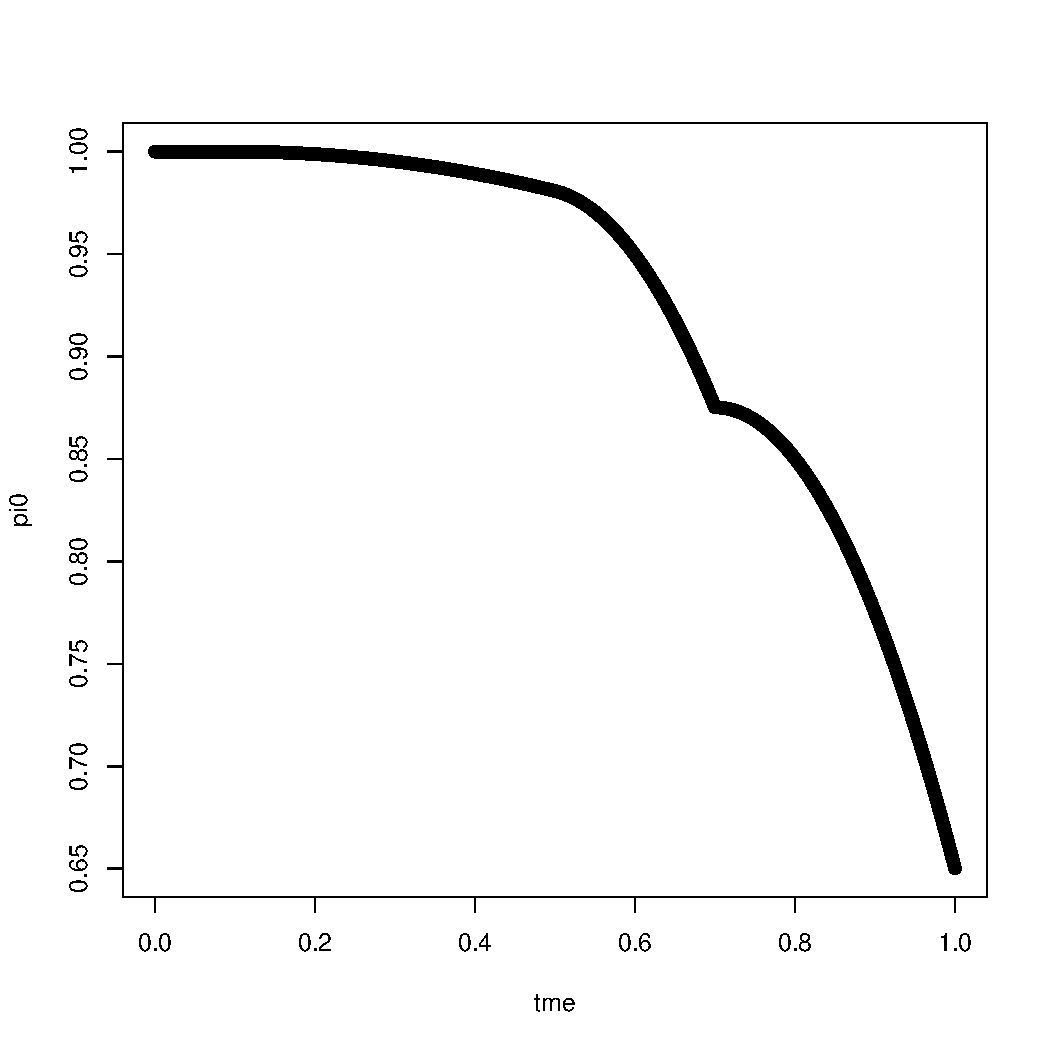
\includegraphics[width=\maxwidth]{Figures/II-1} 

}



\end{knitrout}

\section{Probability of being a false positive is smooth in one variable within levels of second variable}

\begin{knitrout}
\definecolor{shadecolor}{rgb}{0.969, 0.969, 0.969}\color{fgcolor}\begin{kframe}
\begin{alltt}
\hlcom{## Set up the time vector and the probability of being null}
\hlstd{tme1} \hlkwb{<-} \hlkwd{seq}\hlstd{(}\hlnum{0}\hlstd{,}\hlnum{1}\hlstd{,}\hlkwc{length}\hlstd{=ntest)}
\hlstd{tme2cont} \hlkwb{<-} \hlkwd{runif}\hlstd{(ntest,}\hlnum{0}\hlstd{,}\hlnum{0.5}\hlstd{)}
\hlkwd{set.seed}\hlstd{(}\hlnum{309441}\hlstd{)}
\hlstd{tme2} \hlkwb{<-} \hlkwd{rep}\hlstd{(}\hlnum{NA}\hlstd{, ntest)}
\hlstd{tme2[tme2cont} \hlopt{<} \hlnum{0.127}\hlstd{]} \hlkwb{<-} \hlnum{1}
\hlstd{tme2[tme2cont} \hlopt{>=} \hlnum{0.127}\hlstd{]} \hlkwb{<-} \hlnum{2}
\hlstd{tme2[tme2cont} \hlopt{>=} \hlnum{0.302}\hlstd{]} \hlkwb{<-} \hlnum{3}
\hlstd{pi0} \hlkwb{<-} \hlkwd{f}\hlstd{(tme1, tme2)}
\hlkwd{range}\hlstd{(pi0)}
\end{alltt}
\begin{verbatim}
## [1] 0.6503073 1.0000000
\end{verbatim}
\begin{alltt}
\hlkwd{plot}\hlstd{(pi0} \hlopt{~} \hlstd{tme1)}

\hlkwa{for}\hlstd{(alt} \hlkwa{in} \hlstd{alts)}
\hlstd{\{}
  \hlstd{pValuesSims} \hlkwb{<-} \hlkwd{run_sims_alt}\hlstd{(alt, nSims, pi0)}

  \hlkwd{dim}\hlstd{(pValuesSims)}

  \hlstd{zValuesSims} \hlkwb{<-} \hlstd{pValuesSims[,(}\hlnum{2}\hlopt{*}\hlstd{ntest}\hlopt{+}\hlnum{1}\hlstd{)}\hlopt{:}\hlstd{(}\hlnum{3}\hlopt{*}\hlstd{ntest)]}
  \hlstd{nullHypSims} \hlkwb{<-} \hlstd{pValuesSims[,(ntest}\hlopt{+}\hlnum{1}\hlstd{)}\hlopt{:}\hlstd{(}\hlnum{2}\hlopt{*}\hlstd{ntest)]}
  \hlstd{pValuesSims} \hlkwb{<-} \hlstd{pValuesSims[,}\hlnum{1}\hlopt{:}\hlstd{ntest]}

  \hlcom{##save results}
  \hlkwd{save}\hlstd{(}\hlkwc{file}\hlstd{=}\hlkwd{paste}\hlstd{(alt,} \hlstr{"simResults_3.RData"}\hlstd{,}\hlkwc{sep}\hlstd{=}\hlstr{"/"}\hlstd{),}
       \hlkwc{list}\hlstd{=}\hlkwd{c}\hlstd{(}\hlstr{"pi0"}\hlstd{,} \hlstr{"tme1"}\hlstd{,} \hlstr{"tme2"}\hlstd{,} \hlstr{"nullHypSims"}\hlstd{,}\hlstr{"pValuesSims"}\hlstd{,}\hlstr{"zValuesSims"}\hlstd{))}
\hlstd{\}}
\end{alltt}
\end{kframe}

{\centering 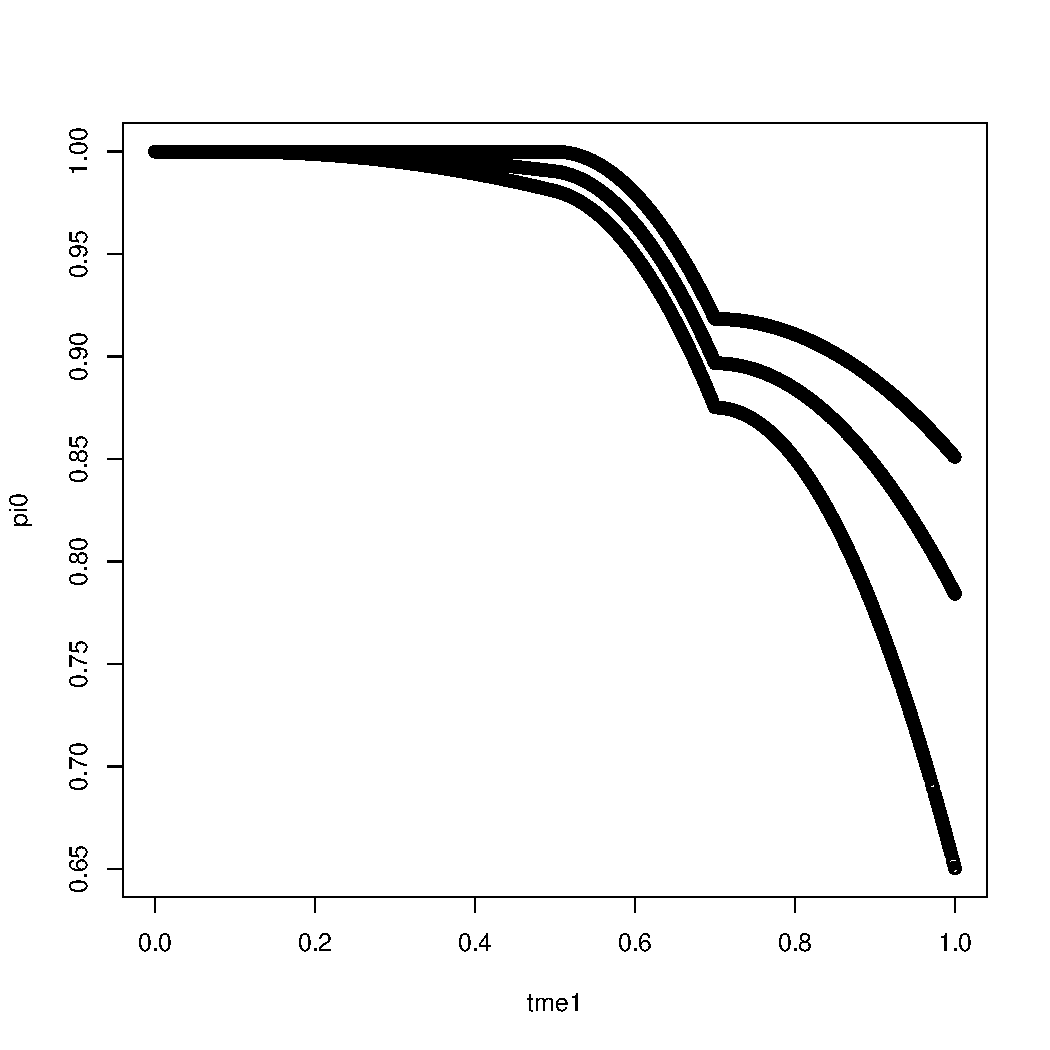
\includegraphics[width=\maxwidth]{Figures/III-1} 

}



\end{knitrout}

\section{Probability of being a false positive is smooth in one variable within levels of second variable - lower priors}

\begin{knitrout}
\definecolor{shadecolor}{rgb}{0.969, 0.969, 0.969}\color{fgcolor}\begin{kframe}
\begin{alltt}
\hlcom{## Set up the time vector and the probability of being null}
\hlstd{tme1} \hlkwb{<-} \hlkwd{seq}\hlstd{(}\hlnum{0}\hlstd{,}\hlnum{1}\hlstd{,}\hlkwc{length}\hlstd{=ntest)}
\hlstd{tme2cont} \hlkwb{<-} \hlkwd{runif}\hlstd{(ntest,}\hlnum{0}\hlstd{,}\hlnum{0.5}\hlstd{)}
\hlkwd{set.seed}\hlstd{(}\hlnum{309441}\hlstd{)}
\hlstd{tme2} \hlkwb{<-} \hlkwd{rep}\hlstd{(}\hlnum{NA}\hlstd{, ntest)}
\hlstd{tme2[tme2cont} \hlopt{<} \hlnum{0.127}\hlstd{]} \hlkwb{<-} \hlnum{1}
\hlstd{tme2[tme2cont} \hlopt{>=} \hlnum{0.127}\hlstd{]} \hlkwb{<-} \hlnum{2}
\hlstd{tme2[tme2cont} \hlopt{>=} \hlnum{0.302}\hlstd{]} \hlkwb{<-} \hlnum{3}
\hlstd{pi0} \hlkwb{<-} \hlnum{0.6}\hlopt{*}\hlkwd{f}\hlstd{(tme1, tme2)}
\hlkwd{range}\hlstd{(pi0)}
\end{alltt}
\begin{verbatim}
## [1] 0.3901844 0.6000000
\end{verbatim}
\begin{alltt}
\hlkwd{plot}\hlstd{(pi0} \hlopt{~} \hlstd{tme1)}

\hlkwa{for}\hlstd{(alt} \hlkwa{in} \hlstd{alts)}
\hlstd{\{}
  \hlstd{pValuesSims} \hlkwb{<-} \hlkwd{run_sims_alt}\hlstd{(alt, nSims, pi0)}

  \hlkwd{dim}\hlstd{(pValuesSims)}

  \hlstd{zValuesSims} \hlkwb{<-} \hlstd{pValuesSims[,(}\hlnum{2}\hlopt{*}\hlstd{ntest}\hlopt{+}\hlnum{1}\hlstd{)}\hlopt{:}\hlstd{(}\hlnum{3}\hlopt{*}\hlstd{ntest)]}
  \hlstd{nullHypSims} \hlkwb{<-} \hlstd{pValuesSims[,(ntest}\hlopt{+}\hlnum{1}\hlstd{)}\hlopt{:}\hlstd{(}\hlnum{2}\hlopt{*}\hlstd{ntest)]}
  \hlstd{pValuesSims} \hlkwb{<-} \hlstd{pValuesSims[,}\hlnum{1}\hlopt{:}\hlstd{ntest]}

  \hlcom{##save results}
  \hlkwd{save}\hlstd{(}\hlkwc{file}\hlstd{=}\hlkwd{paste}\hlstd{(alt,} \hlstr{"simResults_4.RData"}\hlstd{,}\hlkwc{sep}\hlstd{=}\hlstr{"/"}\hlstd{),}
       \hlkwc{list}\hlstd{=}\hlkwd{c}\hlstd{(}\hlstr{"pi0"}\hlstd{,} \hlstr{"tme1"}\hlstd{,} \hlstr{"tme2"}\hlstd{,} \hlstr{"nullHypSims"}\hlstd{,}\hlstr{"pValuesSims"}\hlstd{,}\hlstr{"zValuesSims"}\hlstd{))}
\hlstd{\}}
\end{alltt}
\end{kframe}

{\centering 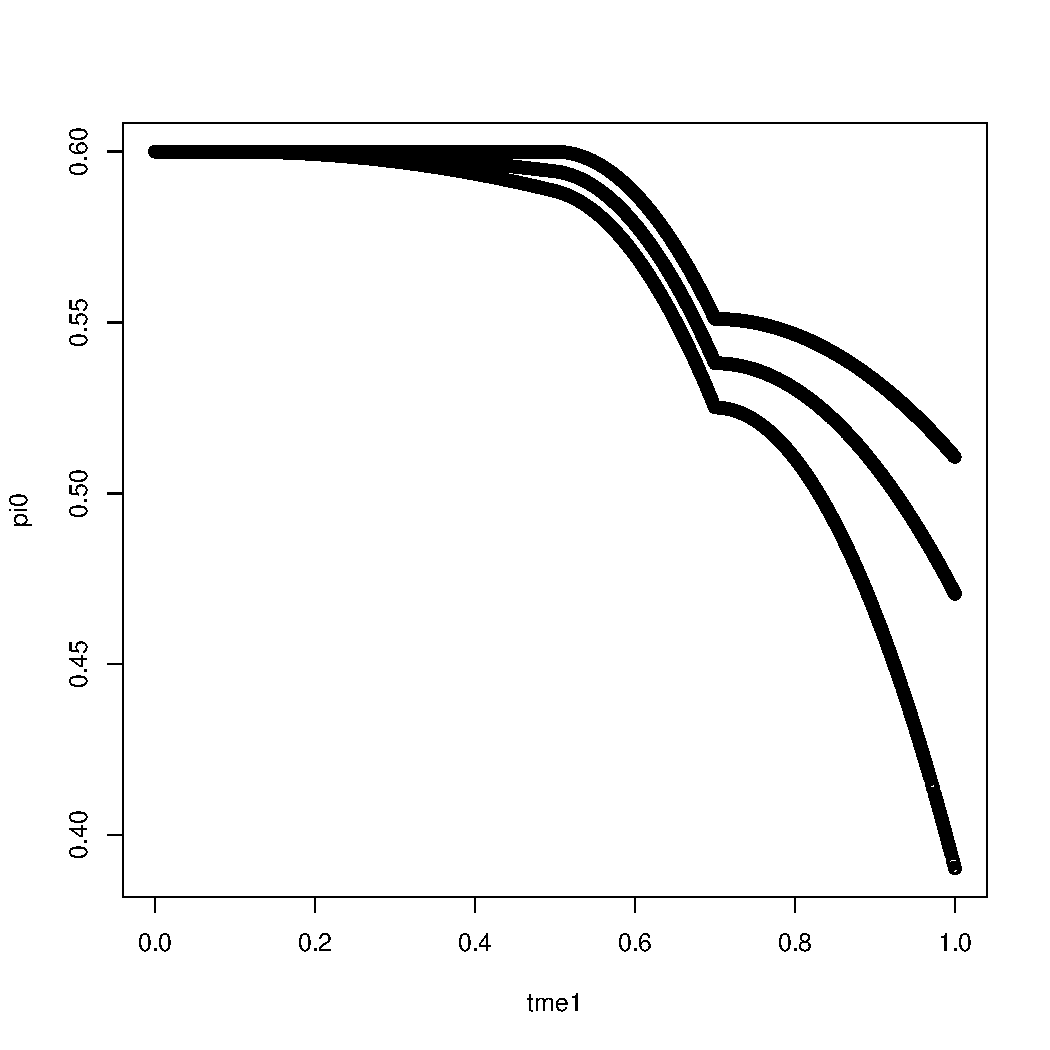
\includegraphics[width=\maxwidth]{Figures/IV-1} 

}



\end{knitrout}

Session info:
\begin{knitrout}
\definecolor{shadecolor}{rgb}{0.969, 0.969, 0.969}\color{fgcolor}\begin{kframe}
\begin{alltt}
\hlstd{devtools}\hlopt{::}\hlkwd{session_info}\hlstd{()}
\end{alltt}


{\ttfamily\noindent\itshape\color{messagecolor}{\#\# Session info -----------------------------------------------}}\begin{verbatim}
##  setting  value                       
##  version  R version 3.4.0 (2017-04-21)
##  system   x86_64, mingw32             
##  ui       RTerm                       
##  language (EN)                        
##  collate  English_United States.1252  
##  tz       America/New_York            
##  date     2017-06-13
\end{verbatim}


{\ttfamily\noindent\itshape\color{messagecolor}{\#\# Packages ---------------------------------------------------}}\begin{verbatim}
##  package    * version date       source        
##  codetools    0.2-15  2016-10-05 CRAN (R 3.4.0)
##  devtools     1.12.0  2016-12-05 CRAN (R 3.4.0)
##  digest       0.6.12  2017-01-27 CRAN (R 3.4.0)
##  doParallel * 1.0.10  2015-10-14 CRAN (R 3.4.0)
##  doRNG      * 1.6.6   2017-04-10 CRAN (R 3.4.0)
##  evaluate     0.10    2016-10-11 CRAN (R 3.4.0)
##  foreach    * 1.4.3   2015-10-13 CRAN (R 3.4.0)
##  highr        0.6     2016-05-09 CRAN (R 3.4.0)
##  iterators  * 1.0.8   2015-10-13 CRAN (R 3.4.0)
##  knitr      * 1.15.1  2016-11-22 CRAN (R 3.4.0)
##  magrittr     1.5     2014-11-22 CRAN (R 3.4.0)
##  MASS       * 7.3-47  2017-02-26 CRAN (R 3.4.0)
##  memoise      1.1.0   2017-04-21 CRAN (R 3.4.0)
##  pkgmaker   * 0.22    2014-05-14 CRAN (R 3.4.0)
##  registry   * 0.3     2015-07-08 CRAN (R 3.4.0)
##  rngtools   * 1.2.4   2014-03-06 CRAN (R 3.4.0)
##  stringi      1.1.5   2017-04-07 CRAN (R 3.4.0)
##  stringr      1.2.0   2017-02-18 CRAN (R 3.4.0)
##  withr        1.0.2   2016-06-20 CRAN (R 3.4.0)
##  xtable       1.8-2   2016-02-05 CRAN (R 3.4.0)
\end{verbatim}
\end{kframe}
\end{knitrout}

\end{document}
